\chapter{Lösungsansatz} 
\label{chapter:Kapitel5}
\lhead{Kapitel 5. \emph{Lösungsansatz}}  

\section{Überblick - Plesynd}
\begin{landscape}
\begin{figure}[ht]
  \centering
  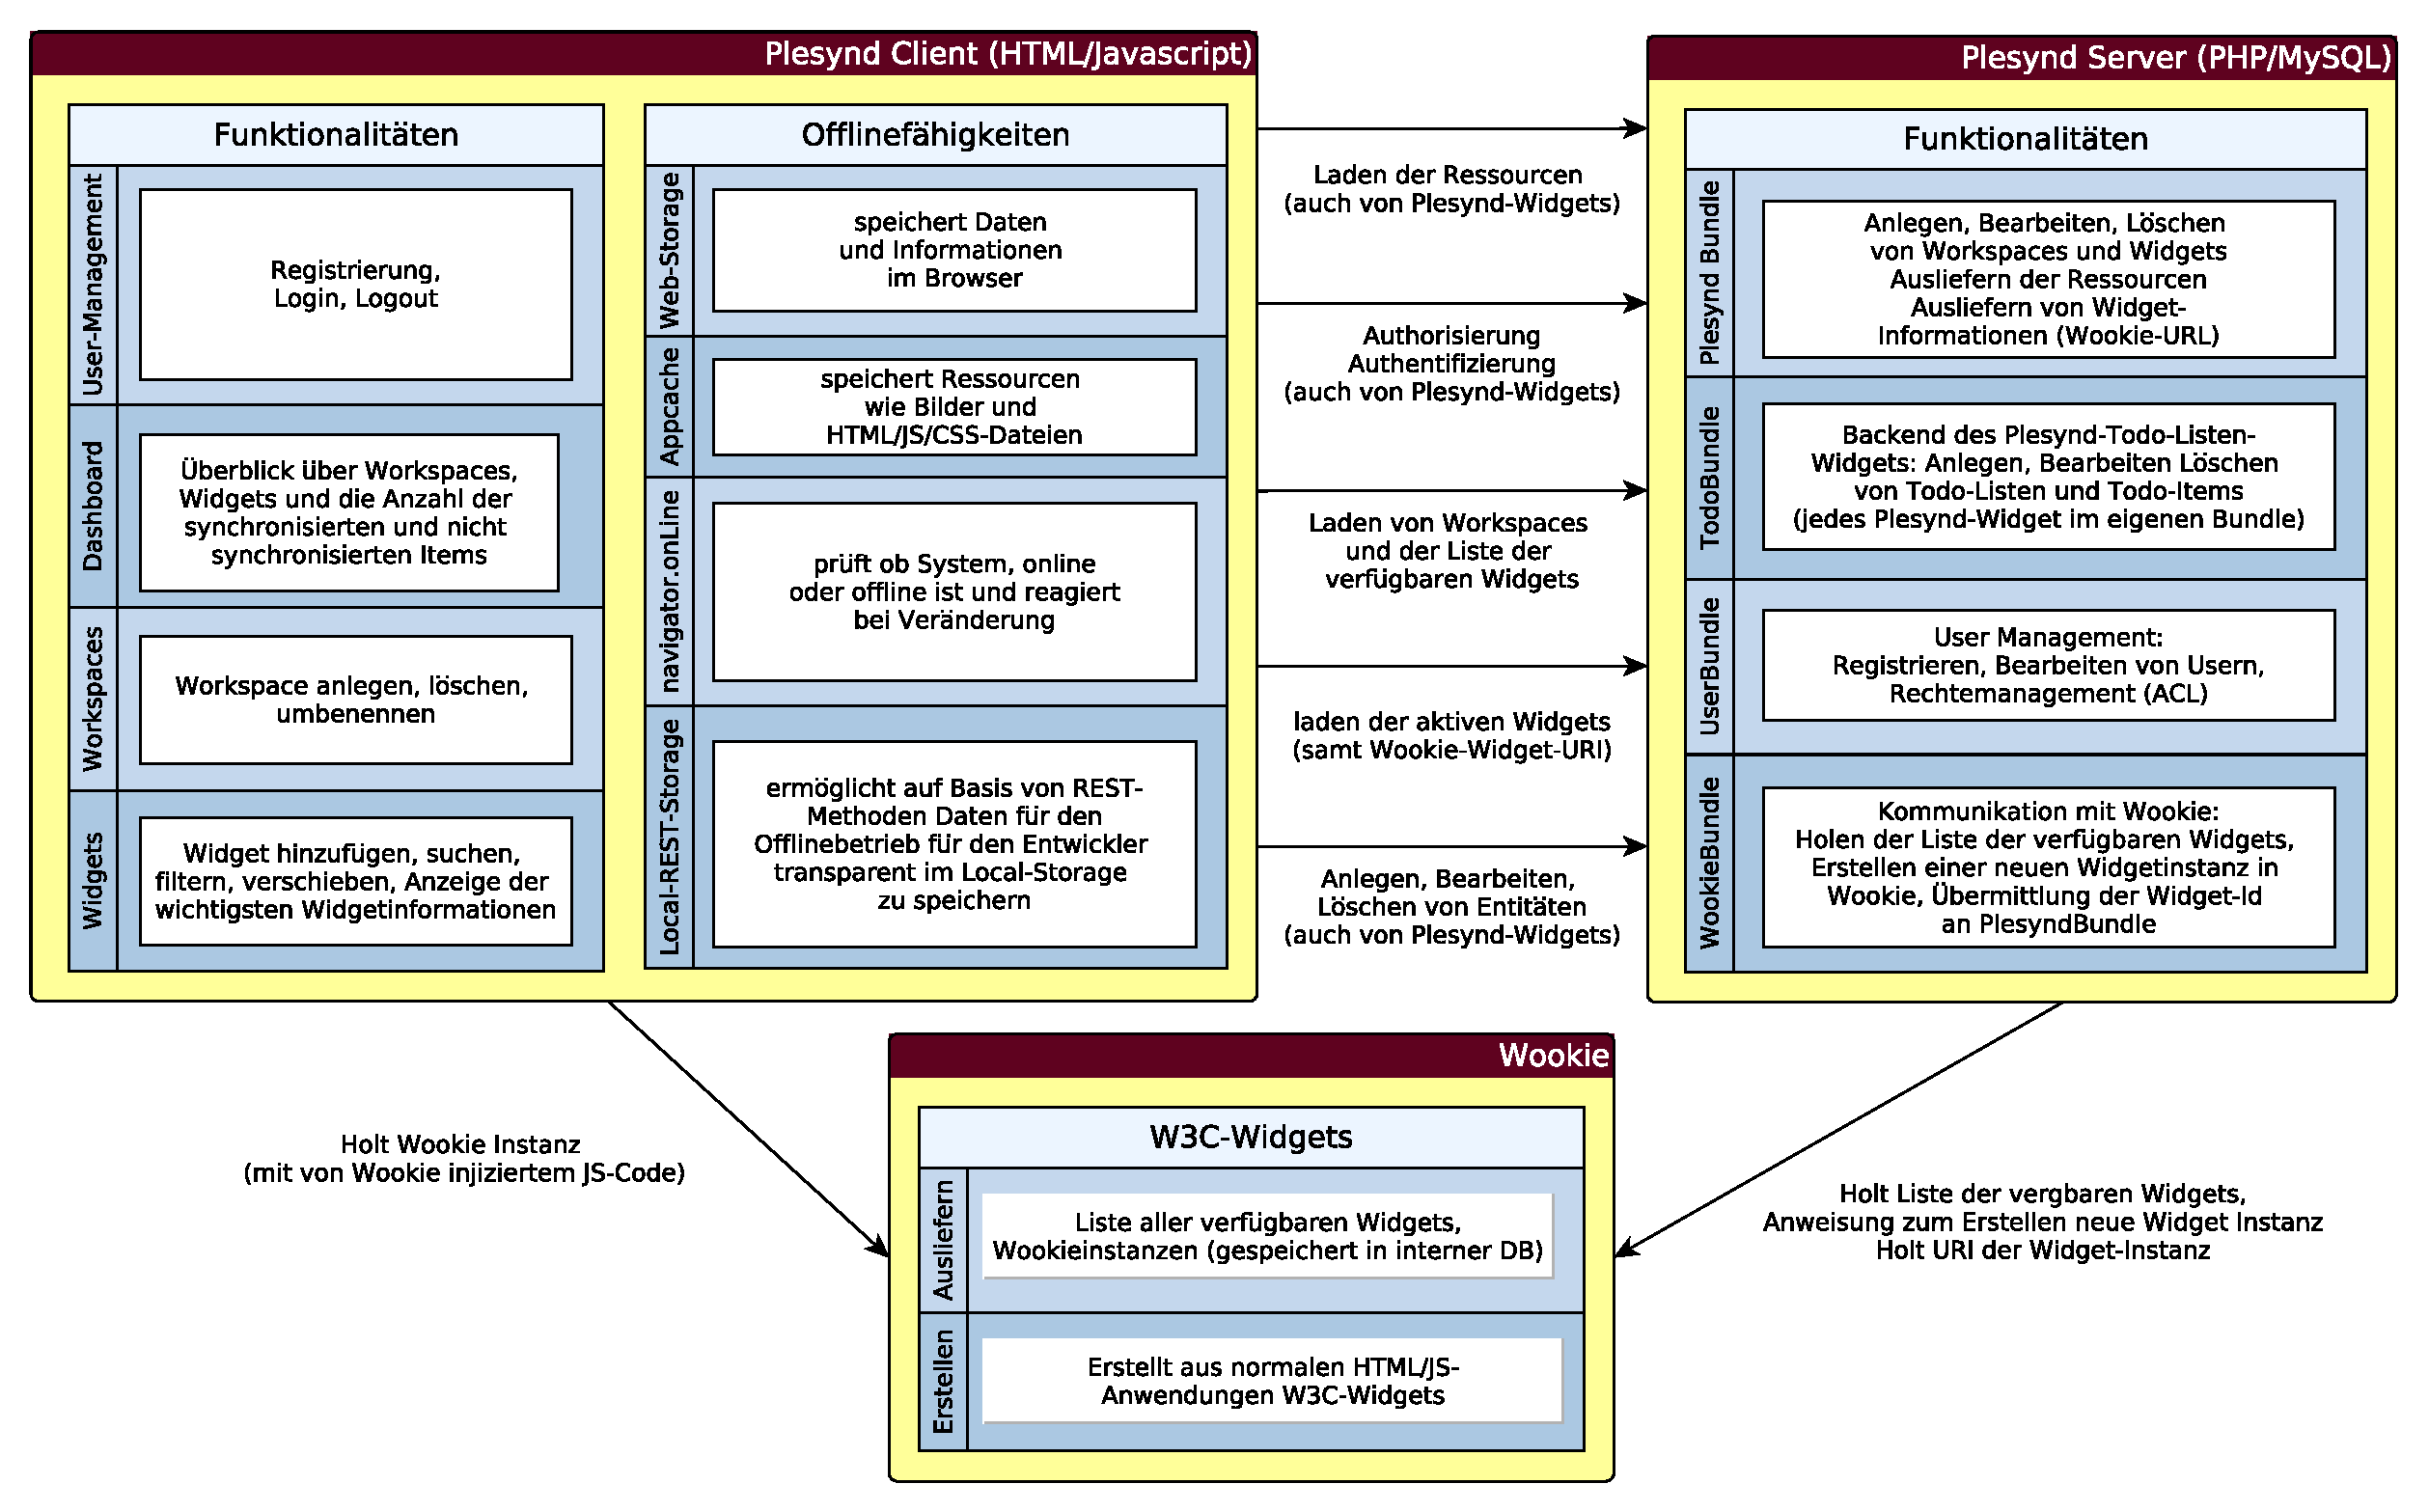
\includegraphics[height=\textheight,keepaspectratio]{./Figures/konzeptionelle_loesung_table.pdf}
    \rule{35em}{0.5pt}
  \caption[Zusammenspiel der wichtigsten Komponenten innerhalb von Plesynd]{Zusammenspiel der wichtigsten Komponenten innerhalb von Plesynd}
  \label{fig:konzeptionelle_loesung2}
\end{figure}
\end{landscape}


Das Ziel dieser Arbeit war die Entwicklung eines leichtgewichtigen Prototypen einer Personal Learning Environment, welcher die Anforderungen aus \ref{section:anforderungen_summary} erfüllt. Für die Umsetzung dieses Ansatzes wurde das Hauptaugenmerk auf die Screen- und die Data-Dimension nach Palmér zu gerichtet (siehe Abschnitt \ref{section:dimensions_palmer}). Die Screen-Dimension, also das User-Interface wird in Abschnitt \ref{section:user_interface} beschrieben. Bei der Umsetzung der Data-Dimension handelt es sich primär um die Implementierung der Online-Offline-Fähigkeit des Systems (siehe Abschnitt \ref{section:technische_umsetzung}).

Der Name des Systems lautet Plesynd (Personal-Learning-Environment Synchronize Data) und wird wie das englische "`pleasant"' (angenehm) ausgesprochen. Plesynd ist ein webbasiertes Dashboard, welches die Möglichkeit bietet mit unterschiedlichen Widgets in Kommunikation zu treten. Wichtig ist hierbei eine Abgrenzung zu zentralisierten Lern-Management-Systemen wie Moodle oder Sakai. Die sind sehr kurszentriert und können auch nur schwer mit den Wilson-Patterns für nutzerzentrierte Personal-Learning-Environment Systeme klassifiziert werden (siehe \ref{section:wilson_patterns}). Aus diesem Grund orientiert sich Plesynd viel stärker an bestehenden Widget-Aggregatoren wie iGoogle oder Netvibes (siehe \ref{section:aehnliche_systeme}). Um dem Nutzer die Möglichkeit zu geben in unterschiedlichen Kontexten mit dem System zu arbeiten und so von dem kurszentrierten Ansatz von LM-Systemen zu dem nutzerzentrierten Ansatz von PLEs zu kommen, wird das System dem Nutzer die Möglichkeit geben, seine Widgets in unterschiedliche Bereiche, sogenannte Workspaces, aufzuteilen. Die Anzahl der Workspaces ist frei und jeder Workspace kann individuell benannt werden.

Der entscheidende Unterschied von Plesynd zu den erwähnten Systemen ist die Offline-Fähigkeit der PLE. Es wurde ein Ansatz entwickelt, der es ermöglicht Widgets so zu implementieren, dass ihre Informationen offline verfügbar gemacht werden. Des weiteren kann auch auch offline mit Plesynd und den Widgets weitergearbeitet werden. Sobald wieder eine Online-Verbindung hergestellt ist, werden die veränderten Daten mit dem Backend synchronisiert.

Das Ziel beim Design von Plesynd war es dem Nutzer die Bedienung so einfach wie möglich zu machen. Die wichtigsten Informationen sollten ihm direkt direkt zur Verfügung gestellt werden (sind alle Daten aktuell, welche Widgets werden benutzt, ist das System offline oder online etc). Widgets können gesucht, nach Offline-Kompatibilität gefiltert und dem System hinzugefügt werden. Es existiert ein Dashboard, welches dem Nutzer anzeigt welche Widgets auf welchen Workspaces zur Verfügung stehen und wie ihr Online-/Offline-Status ist. 

\section{Technische Umsetzung}\label{section:technische_umsetzung}
Plesynd wurde auf der Serverseite mit PHP und auf der Clientseite mit Html5 und Javascript umgesetzt. Die verwendeten Frameworks und zusätzlichen Werkzeuge werden in Kapitel \ref{section:entwicklungsumgebungen_tools} vorgestellt und eingehender beschrieben. Für die Kommunikation mit dem Server verwendet das System REST konforme Anfragen (siehe Kapitel \ref{section:rest}). 
Die Heraustellungsmerkmale von Plesynd sind die Fähigkeit die wichtigsten Funktionalitäten auch offline weiterhin nutzen zu können und die Synchronisierung der Daten, wenn das System wieder online ist. Klassifiziert man diese Fähigkeiten wie in Kapitel \ref{section:klassifizierungsmethoden} beschrieben, so gehören sie in die von Palmér definierte Data-Dimension. Diese Funktionalitäten beschäftigen sich primär mit den Umgang mit Daten und Informationen und den Austausch ebendieser zwischen unterschiedlichen Systemen (zwischen Plesynd und den Widgets) und der Synchronisierung der Daten bei Statusänderung (von Offline- zu Online-Modus). Die Fähigkeit zum Umgang mit unterschiedlichen Status des System kann auch als eine Erweiterung des von Wilson vorgestellten Multimode-Patterns (siehe Seite \pageref{wilson_patterns:multimode}) betrachtet werden. 

Die Möglichkeit Javascript, Css und Html Dateien im Browser zu speichern wurde mit der Html5 Appcache-API umgesetzt (siehe Kapitel \ref{section:appcache}). Sollte einmal eine andere Speichertechnik als der Web-Storage benötigt werden, ist das System so implementiert, dass die Art der lokalen Speicherung losgelöst von der restlichen Anwendung umgestaltet werden kann.

Plesynd erkennt über ein globales Javascript-Event (siehe Kapitel \ref{section:online_offline_erkennung}), wenn sich der Browser in einem Zustand befindet, in dem er keine Konnektivität mit dem Internet besitzt. Das System informiert den User darüber, kann aber auch entscheiden, welche Funktionalitäten es dem Nutzer zur Verfügung stellen darf. Nimmt der Anwender Änderungen an den Daten vor, werden diese nur in den Local-Storage geschrieben. Sobald sich das System wieder mit dem Internet verbindet erkennt Plesynd diese Zustandsänderung und synchronisiert die Daten mit den zugrunde liegenden Services. 

TODO Erstellung einer Grafik mit den Komponenten und Zusammenspiel dieser


Wookie
Plesynd 
W3C

Browser, local storage 

Probleme mit der bei modernen Browser üblichen Same-Origin-Policy für Request wurden mit dem Cross-Origin Resource Sharing (CORS) Mechanismus (siehe \ref{section:same_origin_policy}) und die Postmessage-API (siehe \ref{section:same_origin_policy}) gelöst. 


\begin{lstlisting}
<preference name="plesynd_offline_compatible" value="true"/>
\end{lstlisting}

\section{User Interface}\label{section:user_interface}
Für die Umsetzung der Screen-Dimension, also des User-Interfaces kommen in Plesynd drei wichtige Konzepte zum Einsatz: Dashboard, Widgets und Workspaces. 

Über Widgets werden die unterschiedlichen Werkzeuge und Services, die ein Nutzer innerhalb des Systems nutzen möchte eingebunden (siehe: Kapitel \ref{section:widgets}). Die Umsetzung der einzelnen Widgets liegt in der Hand des jeweiligen Designers. Da Plesynd Wookie als Widget Container benutzt, ist es möglich alle W3C-Widgets in das System einzubinden. Für diese Arbeit wurde ein Todo-Listen-Service entwickelt für den als prototypische Entwicklung ein Widget mit Online-/Offline-Fähigkeiten implementiert wurde. Besitzt ein Widget Online-/Offline-Fähigkeiten so erhält es eine von Plesynd zur Verfügung gestellte Statusleiste, in der der aktuelle Online-/Offline-Status, sowie die Anzahl der verfügbaren Items und der noch nicht synchronisierten Item angezeigt wird (Abbildungen \ref{fig:plesynd_workspace_online} und \ref{fig:plesynd_workspace_offline}).
\begin{figure}
  \centering
  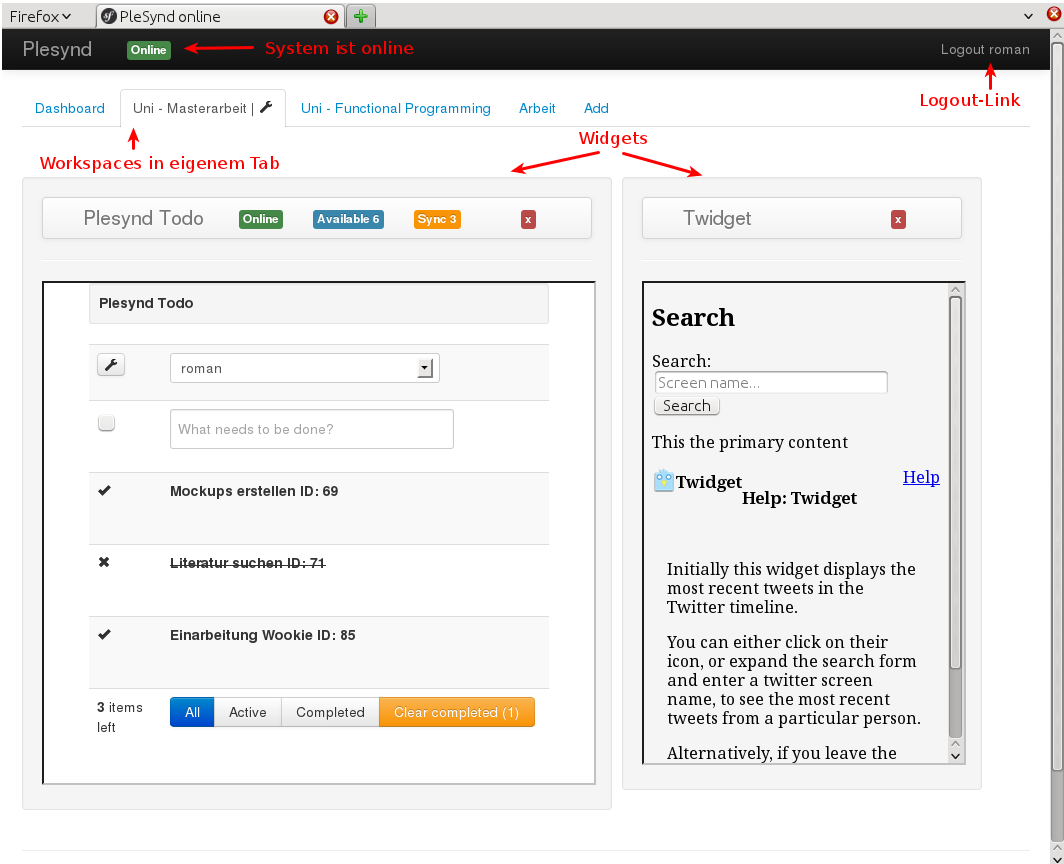
\includegraphics[width=\textwidth,height=\textheight,keepaspectratio]{./Figures/plesynd_workspace_online.png}
    \rule{35em}{0.5pt}
  \caption[Plesynd User-Interface: Workspace Online]{Ein Workspace mit unterschiedlichen Widgets}
  \label{fig:plesynd_workspace_online}
\end{figure}

\begin{figure}
  \centering
  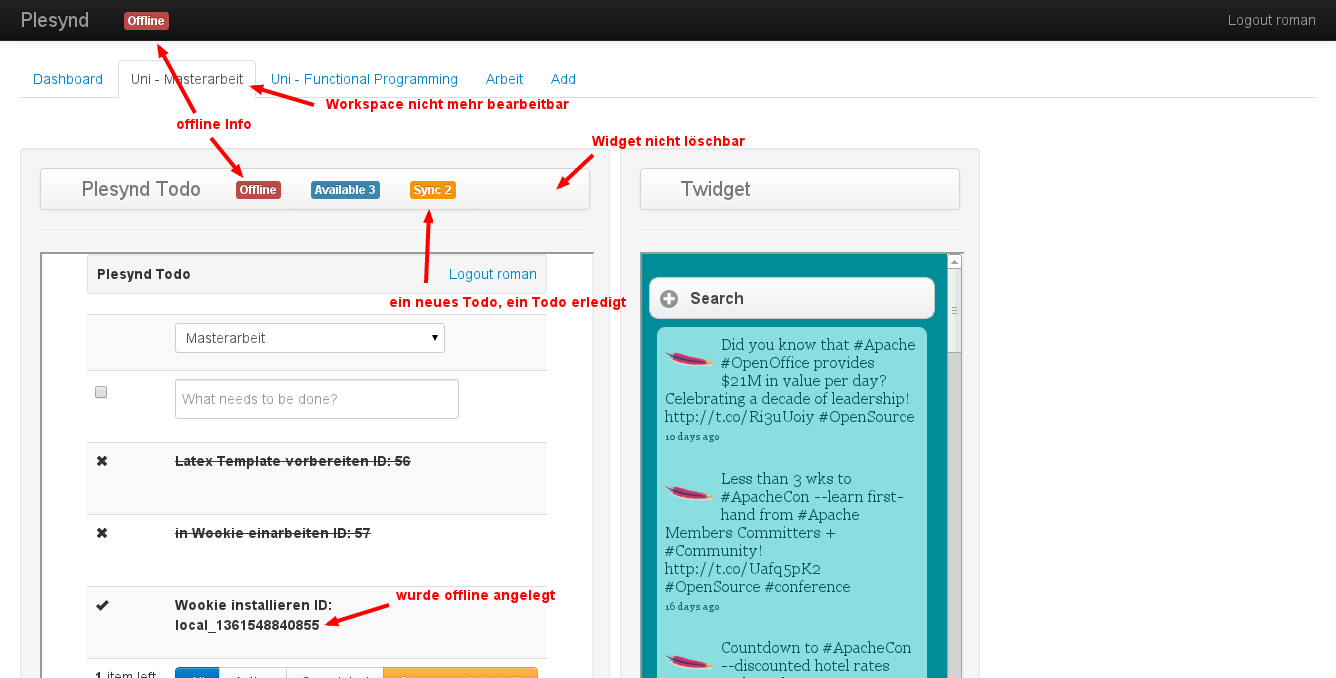
\includegraphics[width=\textwidth,height=\textheight,keepaspectratio]{./Figures/plesynd_workspace_offline.png}
    \rule{35em}{0.5pt}
  \caption[Plesynd User-Interface: Workspace Offline]{Die wichtigsten Unterschiede im Offline-Modus}
  \label{fig:plesynd_workspace_offline}
\end{figure}
Der Nutzer hat die Möglichkeit Widgets nach Themen oder Einsatzgebieten zu gruppieren. Dies geschieht über sogenannte Workspaces. Workspaces sind vom Nutzer frei und in unbegrenzter Zahl hinzufügbare Bereiche im System. Sie sind über eine Reiter-Navigation zu erreichen und können jederzeit umbenannt oder auch wieder gelöscht werden (Abbildung \ref{fig:plesynd_workspace_edit}). 
\begin{figure}
  \centering
  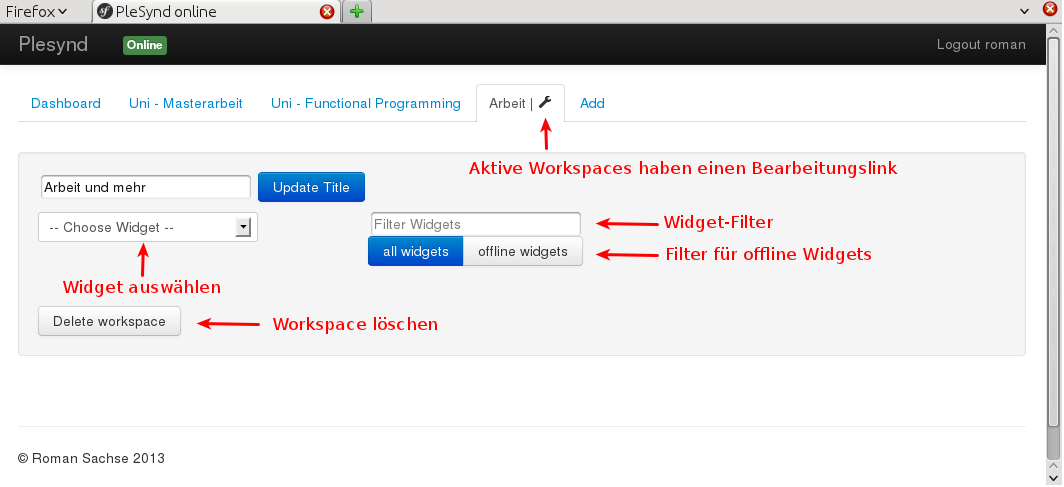
\includegraphics[width=\textwidth,height=\textheight,keepaspectratio]{./Figures/plesynd_workspace_edit.png}
    \rule{35em}{0.5pt}
  \caption[Plesynd User-Interface: Bearbeiten von Workspaces]{Workspaces können direkt bearbeitet werden.}
  \label{fig:plesynd_workspace_edit}
\end{figure}

Jedes Widget kann einem Workspace hinzugefügt werden. Die Position der Widgets innerhalb eines Workspaces kann über einen Drag and Drop Mechanismus angepasst werden. Die Startseite stellt als Dashboard die wichtigsten Informationen dar. Jeder Workspace wird in einer eigenen Tabelle inklusive seiner Widgets und der Anzahl der zur Verfügung stehenden Widgets präsentiert. Über direkte Links innerhalb des Dashboards ist es dem Nutzer möglich direkt zu dem gewünschten Workspace zu navigieren (siehe Abbildung \ref{fig:plesynd_dashboard}.
\begin{figure}
  \centering
  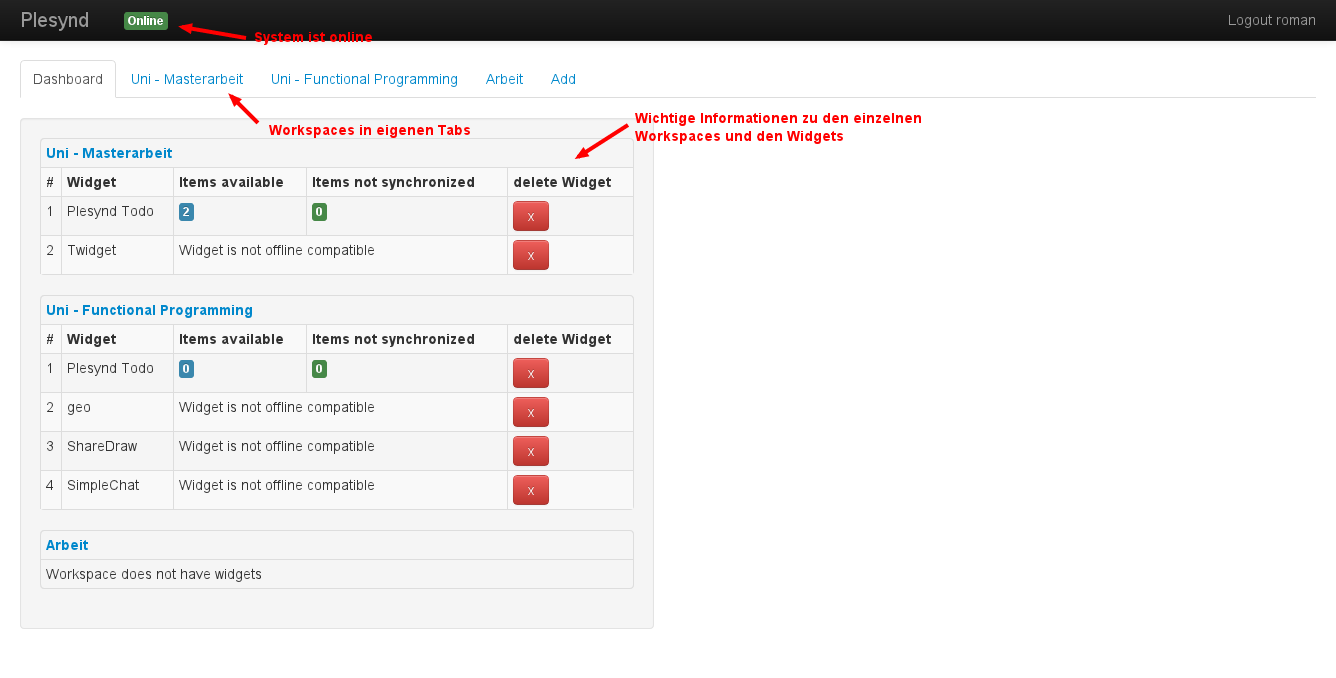
\includegraphics[width=\textwidth,height=\textheight,keepaspectratio]{./Figures/plesynd_dashboard.png}
    \rule{35em}{0.5pt}
  \caption[Plesynd User-Interface: Dashboard]{Das Dashboard fasst die wichtigsten Informationen zusammen.}
  \label{fig:plesynd_dashboard}
\end{figure}

TODO schauen was in 4 noch nicht verwendet wurde
 Als Einstiegspunkt in das System kann ein "`Discourse Monitor"' dienen. Dieser fungiert als eine Startseite welche dem Nutzer die wichtigsten Informationen bezüglich seiner Workspaces und gibt ihm durch Links dorthin die Möglichkeit direkt zu den gewünschten Personal-Learning-Tools zu gelangen. Der "`Navigation Layer"'  ist in Plesynd inhärent mit eingebaut. Durch die Einbindung externer Widgets, wird dem User nur der Funktionsumfang zur Verfügung gestellt, welche von den Widget-Entwicklern angedacht wurde. Für den vollen Funktionsumfang muss der Nutzer zum eigentlichen Service des Widgets navigieren. Die Widgets werden über die vom System zur Verfügung gestellten Workspaces aggregiert und in übersichtlicher Form präsentiert. Der Nutzer ist in der Lage Widgets zu seinen frei definierbaren Workspaces hinzuzufügen, zu entfernen oder über Drag and Drop nach seinen Wünschen anzuordnen. Dadurch wird ist auch das "`Choose Change and Discard"'-Pattern (siehe Seite \pageref{wilson_patterns:choose_change_discard}) grundsätzlich im System verankert.  







